%%Chapter - Split into separate file if too large
\chapter{Main Dishes}
%%Start recipe
\newrecipe{Dukkah Crusted Chicken with Morrocan Tomato Cardomon Sauce}{http://www.taste.com.au/recipes/4743/dukkah_crusted_chicken_with_moroccan_tomato_cardamom_sauce}
\section*{Ingredients}
\begin{ingredients-list}
	\item 50g dukkah
	\item 10 basil leaves, chopped
	\item 2 tbsp. grated orange rind
	\item 6 (about 130g each) skinless chicken breasts
	\item 1 cup (250ml) buttermilk
	\item \sfrac{1}{2} cup (125ml) reduced-salt chicken stock
	\item Juice of 1 orange
	\item Lemon wedges, to serve
\end{ingredients-list}
Moroccan tomato \& cardamom sauce
\begin{ingredients-list}
	\item 2 tbsp. olive oil
	\item 1 large onion, finely chopped
	\item 3 garlic cloves
	\item 3cm piece ginger, grated
	\item 2cm piece fresh turmeric*, grated
	\item 8 green cardamom pods, lightly crushed
	\item 2 kaffir lime leaves
	\item 1 cinnamon stick
	\item 5 roma tomatoes, peeled, seeds removed, finely chopped
	\item 400g canned chopped tomatoes
	\item 2 tsp. palm sugar 
\end{ingredients-list}

\section*{Directions}
\begin{enumerate}
\item For the sauce, heat the olive oil in a pan over medium heat; add the onion and cook, stirring occasionally, until tinged golden. Add the garlic, ginger, turmeric and salt, and then cook for 1-2 minutes, stirring. Add cardamom, kaffir lime leaves, cinnamon stick, and the fresh and canned tomatoes. Cook for 20-25 minutes, stirring occasionally, until thickened.
\item Add palm sugar and season to taste. Remove, discard the kaffir lime leaves and cinnamon, and set aside.
\item Preheat the oven to 180°C.
\item Combine the dukkah, basil and orange rind in a bowl. Dip the chicken breasts in buttermilk, and then roll in the dukkah mixture.
\item Place in a shallow baking dish and pour the chicken stock and orange juice around the chicken. Bake in the oven for 30 minutes or until just cooked through and browned.
\end{enumerate}
To serve, slice each chicken breast into 4 pieces and fan out on plates. Serve with lemon wedges and a dollop of the sauce. 

%%End recipe

%%Start Recipe
\newrecipe{Beef Paprikash}{http://www.abc.net.au/passions/current/cp10w006.htm}

\section*{Ingredients}
Paprikash
\begin{ingredients-list}
	\item 750g chuck steak,
	\item fat trimmed off, cubed
	\item 1 large of 2 medium onions,
	\item finely sliced
	\item 2 tbsp. plain flour seasoned
	\item with white pepper
	\item 2 or 3 tbsp. oil
	\item 150g button mushrooms, wipe clean
	\item 2 or 3 tsp. Hungarian paprika,
	\item depending on strength
	\item 1 tsp. Dijon-style mustard
	\item 1 tsp. sugar
	\item 500ml veal, chicken or vegetable stock
	\item 2 tbsp. sour cream (or crème fraiche)
\end{ingredients-list}
Cabbage
\begin{ingredients-list}
	\item \sfrac{1}{2} small cabbage
	\item with outer leaves removed
	\item 50g bacon cut into small pieces
	\item 2 tsp. olive oil
	\item 2 or 3 tsp. white mustard seeds
\end{ingredients-list}

\section*{Directions}
Paprikash
\begin{enumerate}
	\item Dust steak with the seasoned flour.
	\item In a large saucepan, brown in half the oil over very high heat (do not allow to stew).
	\item Remove to a bowl with slotted spoon or tongs.
	\item In the same pan, brown the mushrooms, and remove to bowl (adding more oil if necessary).
	\item Fry the onion until well cooked and browned.
	\item Stir in paprika and cook a further minute or so.
	\item Add mustard and sugar. Stir in.
	\item Add stock and stir in. Add sour cream and stir in. Fold in beef and mushrooms.
	\item Turn down heat, put on lid and allow to simmer very slowly.
\end{enumerate}
Cabbage
\begin{enumerate}
	\item Cut cabbage into thin slices, remove hard core.
	\item Fry mustard seeds gently in the oil until they start popping.
	\item Stir in bacon, and cook two minutes. Stir in cabbage leaves.
	\item Allow cabbage to cook for 5 or 6 minutes over medium heat, tossing from time to time.
\end{enumerate}
Degree of difficulty: Low
Keepability: Paprikash keeps for a couple of days in the refrigerator. Cabbage is best eaten immediately.
Wine companion: Full bodied red wine, Shiraz or Cabernet Sauvignon.
%%End recipe

%%Start Recipe
\newrecipe{Poh's Nonya Chicken Curry}{http://www.abc.net.au/tv/pohskitchen/stories/s2984186.htm}

\section*{Ingredients}
\begin{ingredients-list}
	\item 3 tbs coriander seeds
	\item 1 tsp cumin seeds
	\item 1 tsp fennel seeds
	\item 15 dried chillies, deseeded, soaked in hot water, drained and chopped
	\item 270g red eschallots, roughly chopped
	\item 3 cloves garlic
	\item 20g belachan, toasted* 
	\item 25g fresh turmeric root
	\item 3 tbs coconut cream
	\item 6 - 7 sprigs of curry leaves
	\item 4 tbs veg oil
	\item 1 star anise
	\item 2 whole cloves
	\item 1 cinnamon stick
	\item 1\sfrac{1}{2} kg chicken thigh fillets
	\item 300g baby chat potatoes peeled and halved
	\item 2 birds eye chillies, de-seeded and halved lengthways
	\item 400ml coconut milk
	\item 1 tbs salt
	\item 1 tsp sugar
	\item 100ml coconut cream
	\item 2 pandan leaves, shredded lengthways and knotted
\end{ingredients-list}

\section*{Directions}
\begin{enumerate}
	\item To begin making the curry, dry toast the coriander, cumin and fennel seeds in a frypan until fragrant and beginning to smoke
		 Tip into mortar and pestle or electric spice grinder and grind to a powder. Set aside.
	\item To make the spice paste or rempah you may do it the old fashioned and very very effective way or blitz the ingredients in a mini food processor.
		If you are using the mortar and pestle, start by pounding a small amount of the prepared, dried chillies and adding small handfuls at a time, all the while pounding thoroughly to a 			fine paste. Continue to add and pound the eschallots, garlic, belachan and turmeric in the same manner until all are a homogenous, fine paste.
		If using a mini food processor still exercise the same patience and pulverize only small amounts of the ingredients at a time, to achieve a fine paste.
	\item Heat vegetable oil in a heavy based saucepan or wok, to a medium heat. Toast star anise, cloves and cinnamon stick for about 20 seconds.
		Add spice paste and sauté for about six to ten minutes, or until the sauce is very fragrant and the oil is separating from the rempah.
		Add coconut cream, pandan leaves and curry leaves and keep cooking until very fragrant.
		You will know when the paste is ready when the oil begins to separate from the mixture and rising to the surface.
	\item Add chicken pieces and stir for one minute. Add potatoes, coconut milk, salt and sugar.
		Cover and simmer until chicken and potatoes are tender. Add coconut cream and birds eye chillies and simmer for a further five minutes.
		Serve with roti and or steamed jasmine rice.
\end{enumerate}
* Shortcut – Toast belachan in a toaster. Note: turn electricity off before retrieving your foil. Simply chop the belachan as finely as possible, scatter thinly onto a double layer foil, fold into a tidy flat parcel and press down slightly all over. Toast in a regular toaster a few times until the belachan is fragrant , dry and crumbly.
%%End Recipe

%%Start recipe
\newrecipe{Lime and cumin chargrilled chicken with mango chilli salsa}{http://www.taste.com.au/recipes/34185/lime+and+cumin+chargrilled+chicken+with+mango+chilli+salsa}
\section*{Ingredients}
\bigskip
\begin{ingredients-list}
	\item 1 cup basil leaves
		\begin{textblock*}{8cm}(7.5cm,-0.8cm) % {block width} (coords)
			\includegraphics[scale=0.39]{./img/lime_cumin_chicken.jpg}
		\end{textblock*}
	\item 1 tbsp cumin seeds, toasted
	\item 2 garlic cloves, crushed
	\item Juice of 1 lime
	\item Grated zest of 2 limes
	\item 2 mangoes, sliced
	\item 1 cup mint leaves
	\item 1 tbsp olive oil
	\item 1 long red chilli, thinly sliced
	\item \sfrac{1}{4} tsp salt
	\item 1 large Coles RSPCA Approved whole chicken, cut into 4 pieces
\end{ingredients-list}

\section*{Directions}
\begin{enumerate}
	\item Preheat oven to 210°C or 190°C fan. Use a mortar and pestle to pound garlic, cumin seeds and salt until a coarse paste forms.
		Stir in lime zest, lime juice and oil. Rub all over chicken.
	\item Preheat an ovenproof chargrill pan on high. Cook the chicken, skin-side down, for 2-3 mins or until charred. Turn and cook for 1 min to seal.
		Place pan in oven and bake for 30 mins or until chicken is cooked through.
	\item Combine the mango, chilli, basil and mint in a bowl. Cut the chicken into smaller pieces and transfer to a platter. Drizzle over the pan juices and serve with the salsa.
\end{enumerate}
 

%%End recipe

%%Start recipe
\newrecipe{Lamb and Cardomom Pilaf}{}
\section*{Ingredients}
\bigskip
\begin{ingredients-list}
	\item 1kg lamb, 2-3cm dice
%%		\begin{textblock*}{8cm}(7.5cm,-0.8cm) % {block width} (coords)
%%			\includegraphics[scale=0.39]{./img/lime_cumin_chicken.jpg}
%%		\end{textblock*}
	\item 1 tsp curry powder
	\item 1 brown onion,diced
	\item 150 grams celery, diced
 	\item 150 grams (about 1) carrot, peeled and diced
	\item 2 cloves garlic, finely chopped
	\item 1 tbsp grated fresh ginger
	\item 1\sfrac{1}{2} cup basmati rice
	\item 150 ml dry white wine
	\item 750 ml warm chicken stock
	\item 1 tsp cardomom seeds
	\item 50 grams butter (optional)
	\item 2 tbsp chopped parsley
	\item 1 tbsp chopped mint
\end{ingredients-list}

\section*{Directions}
\begin{enumerate}
	\item  In a bowl, toss the cubes of lamb in the curry powder and place in the refrigerator for 2 hours.
		When you are ready to cook remove the bowl from the fridge and reheat oven to 160°C or 150°C fan forced.
	\item Warm 2 tbsp olive oil over a medium heat and add the chopped onion, carrot, celery and garlic.  Cook for about 10 minutes until softened but not browned.
		Remove the vegetables from the pot and set aside.
	\item In the same pot over medium high heat brown the lamb in 2 tablespoons of olive oil. Add the grated ginger and season with salt and pepper.
	\item Turn the heat down, and add the cooked vegetables, the rice, the wine, the chicken stock and the caramon seeds to the  pot. Stir, season witha littl esalt and pepper and bring just to the 					boil.
	\item Cover the disk and place in the oven for around 45 minutes, or until all the liquid has been absorbed.
	\item To finish, add the butter (if using) and fluff the pilaf with a fork. Sprinkle over the chopped parsley and mint and serve immediately.
\end{enumerate}

%%End recipe


%%Start recipe
\newrecipe{Laksa}{http://www.taste.com.au/recipes/6388/laksa}
\section*{Ingredients}
\bigskip
\begin{ingredients-list}
	\item 1 tablespoon peanut oil
 	\item 750ml (3 cups) Campbell's Real Stock Chicken
		\begin{textblock*}{11cm}(9.0cm,0.1cm) % {block width} (coords)
			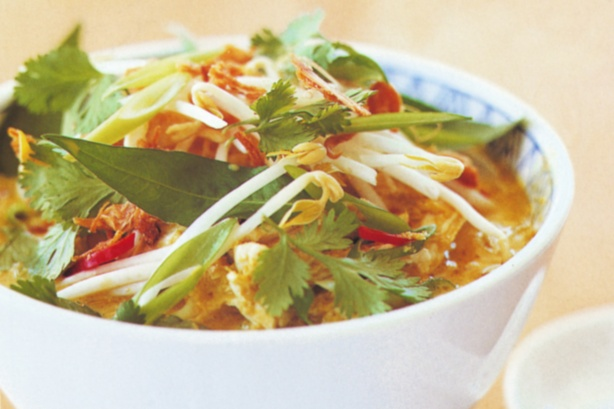
\includegraphics[scale=0.34]{./img/laksa.jpg}
		\end{textblock*}
	\item 500ml (2 cups) coconut milk
	\item 300g pkt dried rice noodles
	\item 2 single chicken breasts, steamed, sliced
	\item 1 pkt bean sprouts, straggly ends trimmed
	\item 4 spring onions, diagonally sliced
	\item 1/2 cup Vietnamese mint leaves
	\item 1/2 cup coriander leaves
	\item Fried eschallots, to serve*
\end{ingredients-list}
Laksa paste
\begin{ingredients-list}
	\item 4 large dried chillies, soaked in hot water
	\item 3 eschallots, preferably Asian (red), peeled, chopped
	\item 2 garlic cloves
	\item 3cm piece fresh ginger
	\item 2 small red chillies, seeded, chopped
	\item 4 stems lemongrass (white part only), sliced
	\item 8 macadamia nuts
	\item 1 teaspoon shrimp paste
	\item 2 teaspoons ground turmeric
	\item 2 teaspoons ground coriander
	\item 1 teaspoon palm or brown sugar
	\item 3 tablespoons peanut oil
\end{ingredients-list}

\section*{Directions}
\begin{enumerate}
	\item  To make the laksa paste, drain the chillies and place in a food processor with the eschallots, garlic, ginger, red chillies, lemongrass, nuts, shrimp paste, turmeric, coriander, sugar and 			peanut oil.  Whiz in the processor until everything is finely chopped and forms a paste. This paste can be kept in a glass jar in the fridge until needed.
	\item Heat the peanut oil in a wok over medium heat. Add the spice paste and stir-fry for about 5-6 minutes until fragrant.
	\item Add the chicken stock and coconut milk, and stir to combine. Bring to the boil, then decrease heat to medium-low and simmer for 5 minutes, stirring occasionally.
	\item Meanwhile, soak the dried rice noodles in a large bowl of boiling water for about 5 minutes until soft. Drain. Divide the noodles among serving bowls and place chicken on top.
		Ladle over the hot soup.
	\item Garnish with the bean sprouts, spring onions, Vietnamese mint leaves, coriander and fried eschallots.
\end{enumerate}
 

%%End recipe

%%End Chapter